\section{Introduction}\label{sec:intro}
Search and rescue (SAR) in protected areas is frequent and time-critical. The parks managed by the U.S. National Park
Service recorded 2\,890 SAR incidents in 2017, and an average of 11.2 per day over 1992--2007
\cite{heggie2009}\todo{verify both numbers on the full text; add a source for Vietnam}. Survival falls quickly with time:
among lost persons with dementia in Virginia, all of those found within 12\,h survived, whereas a third of those found
after 24\,h did not \cite{koester1998}. Searchers start from a last-seen point and expand outwards on foot, with dogs
and with aircraft; in a lowland tropical forest the canopy hides the ground from the air, and visual search from above
is of little use.

Meanwhile, forests are being instrumented. Camera traps are a standard tool of wildlife monitoring, and networked
camera traps now send images over 4G with solar power, e.g., 65 cameras on 34\,km$^2$ of a Natura~2000 site
\cite{kissling2024}. Wildfire sensors form LoRa meshes of about one node per hectare in pilot sites, and one vendor
reports more than 30\,000 deployed sensors \cite{dryad}; GreenOrbs ran up to 330 IEEE 802.15.4 nodes in a forest
\cite{liu2013greenorbs}. Some of these devices, or an edge box next to them, can run a person detector or a
re-identification network. A person lost in such a forest may thus have walked past a device that recorded them, but no
device knows whom to look for, and the forest core has no cellular coverage through which the footage could be
uploaded. We therefore push a compact query down to the devices instead of pulling footage up. Because different
vendors run different embedding models whose vectors are not comparable \cite{shen2020}, the query carries reference
images, $L=12$ images or about 400\,kB, so that each AI node embeds them with its own model.

\begin{figure}[t]\centering
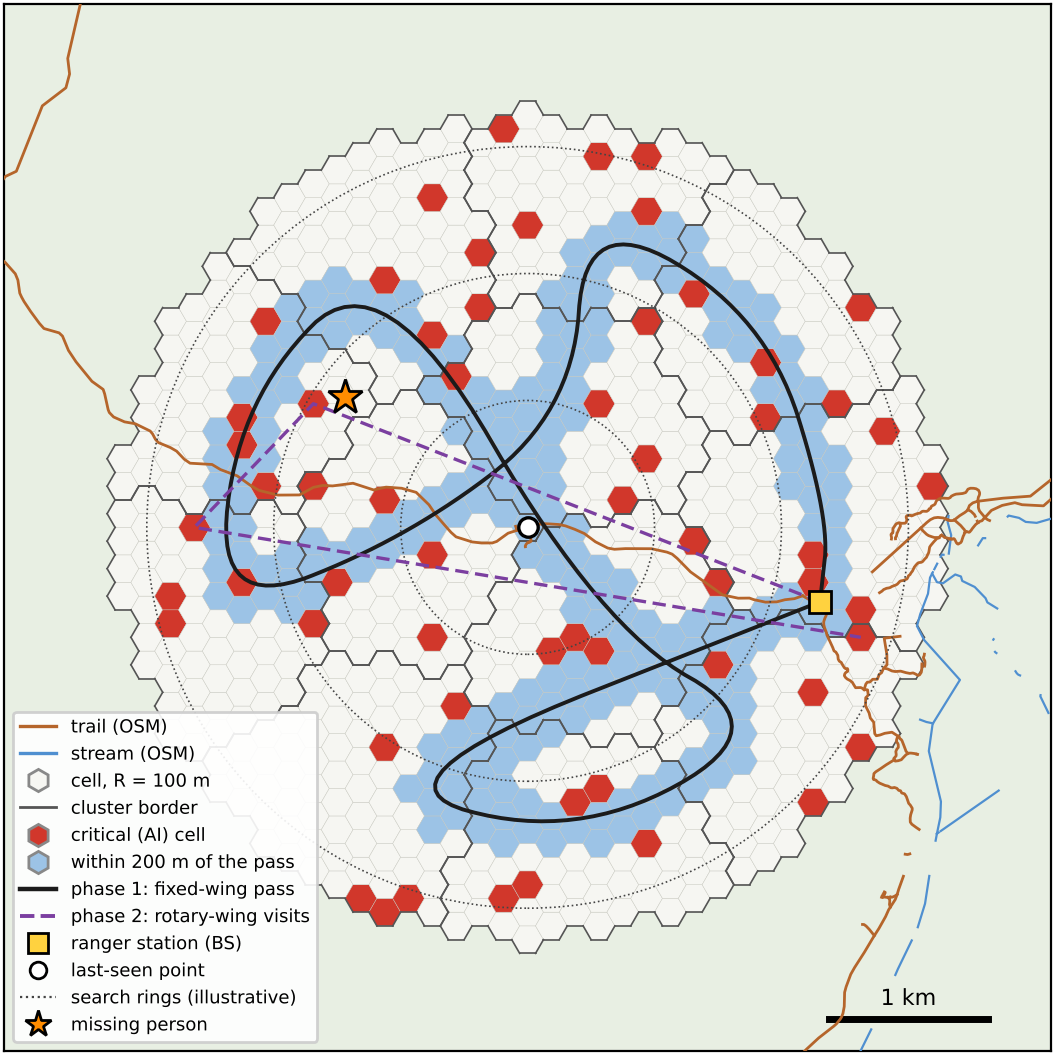
\includegraphics[width=\columnwidth]{draft2-scenario-cattien-labelled.png}
\caption{Scenario on a $6.6\times6.6$\,km window of Cat Tien National Park, Vietnam (trails and streams from
OpenStreetMap). The network around the last-seen point is tiled into cells of radius 100\,m grouped into 12 clusters;
60 cells host an AI node. One fixed-wing pass from the ranger station (phase~1) reaches the cells within about 200\,m
of its track; the ground network carries the query to the remaining AI cells. After the AI nodes report, a rotary-wing
UAV visits the suspected cells (phase~2). Clusters, AI cells, paths and rings are illustrative.}\label{fig:scenario}
\end{figure}

\textbf{Why existing means fall short.} The query cannot travel over LoRa: at spreading factor~7 under a 10\,\% duty
cycle, 400\,kB need at least 1.8\,h of airtime, and 18\,h under a 1\,\% duty cycle, even if every cluster head is in range
of the station. It cannot travel over the 802.15.4 mesh from the station either: the station sits at the forest edge,
the AI nodes are 50--95 radio hops away on our maps, and the measured rates of bulk dissemination protocols translate
into 20\,min to more than an hour at that depth \cite{liang2008,du2017}\todo{redo the hop count on the forest maps}. A
fixed-wing UAV can fly over the forest in minutes and broadcast the query, but it cannot hover and crosses each cluster
once. Under the canopy the air-to-ground (A2G) range of 802.15.4 drops to 100--200\,m (Section~\ref{sec:model}), so a
cell hears only the few hundred packets emitted while the UAV is overhead, and the AI nodes, which are rarely on the
track, cannot assemble the query alone. Making the UAV dwell above every AI node until it has decoded a rateless code
\cite{zeng2018multicast} costs airtime at every receiver: in our conference version we proved that every scheme in
which a device relies only on what its own cell hears from the UAV needs at least the query airtime multiplied by a
fractional covering number of the AI cells, which reaches 35--76 at 100\,m range on our maps (Fig.~\ref{fig:bound}).

\begin{figure}[t]\centering
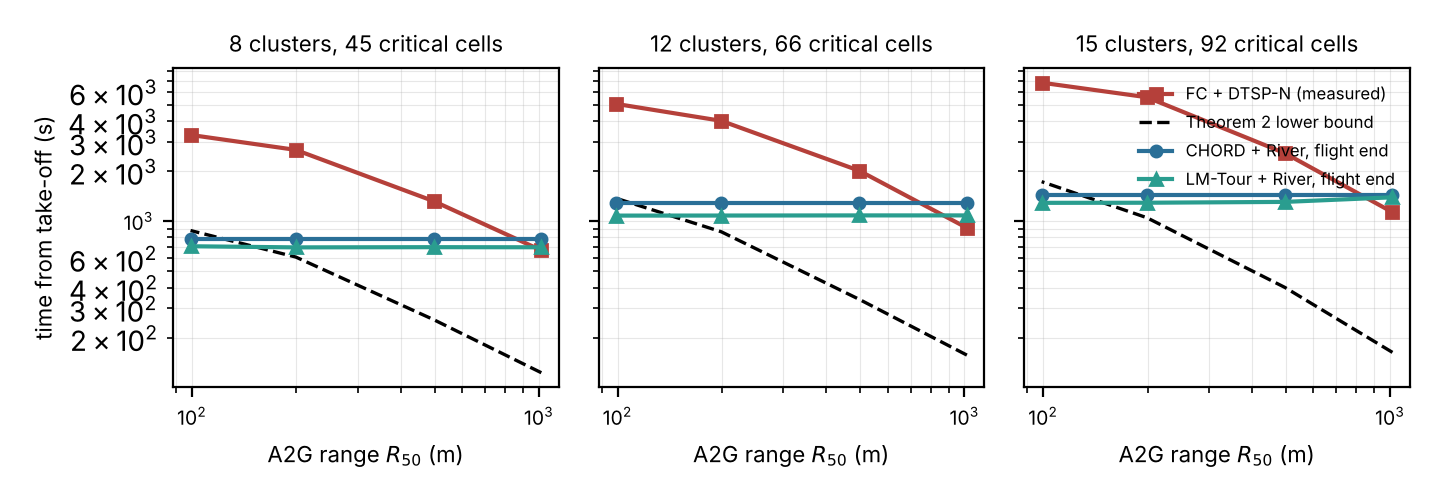
\includegraphics[width=\columnwidth]{bound-nc.png}
\caption{Why direct reception fails under the canopy. Time from take-off on three synthetic forest maps versus the A2G
range $R_{50}$. Red: fountain-coded loitering (FC + DTSP-N), measured in ns-3. Dashed: lower bound for every
non-cooperative scheme. Blue and green: the time at which the planned-cooperation flights end. \todo{redraw for the
forest maps with labels in the paper style.}}\label{fig:bound}
\end{figure}

\textbf{Key insight.} Packet $s$ of the broadcast is emitted at a point of a flight path that the base station designs.
Before take-off the station therefore knows which segment of the stream lands on which cell, and can plan the ground
cooperation that carries the missing segments to the AI nodes: the flight geometry is the transmission schedule.

\textbf{Three phases and their trade-offs.} We organise a mission into three phases (Fig.~\ref{fig:phases}). Phase~0
runs offline: the station selects the cells that host AI nodes and the assignment of the other devices to them, and
precomputes flight and ground plans. Phase~1 starts with the incident: a fixed-wing UAV broadcasts the query in one pass
and the ground network carries the missing parts to the AI cells, which match the query against their stored detections
and report over LoRa. Phase~2 sends a rotary-wing UAV to verify the suspected cells in an order driven by the posterior
probability of the person's location. The phases trade against each other. More AI cells shorten the paths of the
background data from the devices to their AI node, but give phase~1 more cells to serve and phase~2 more false alarms;
a flight that passes close to every AI cell is longer; and the order in which phase~1 serves the clusters decides when
phase~2 learns where to go.

\textbf{Objective.} We minimise the 0.9-quantile of the time $T^\star$ from take-off until the person is confirmed,
subject to the background-traffic budget, the hop limit and memory of the AI nodes, the energy of battery-powered
devices and the endurance of both UAVs. We report the mean as well.

\textbf{Contributions.} This paper extends our conference version \todo{cite ICC 2027 submission} as follows.
\begin{enumerate}
\item \emph{Scenario and model.} A model of query delivery in a lowland forest, with A2G and ground links attenuated by
foliage, battery-powered devices and a prior on the person's location (Sections~\ref{sec:system}--\ref{sec:model}). We
report the device densities of real forest deployments and state openly that our density is a forward-looking
assumption.
\item \emph{Formulation and complexity.} Three core problems, one per phase: (P0) a single-source capacitated facility
location problem with hop and congestion constraints; (P1) a Dubins traveling salesman problem with neighbourhoods
coupled with a time-expanded multicommodity flow on unit-capacity media; and (P2) an online latency-type routing
problem. (P1) is NP-hard already without ground links, and we identify the known hard problems that (P0) and (P2)
contain (Section~\ref{sec:problem}).
\item \emph{Limits.} \todo{Section VI: covering bound for non-cooperative delivery, single-radio and LP bounds for the
ground transport, restated for the forest model.}
\item \emph{Algorithms.} \todo{Section VII: AI-cell selection, \chord{}/\lmtour{}, load-balanced \river{} with shared
trees, takeover with adaptive radius, phase-2 policy.}
\item \emph{Evaluation.} \todo{Section VIII: ns-3 with a full 802.15.4 MAC on forest maps.}
\end{enumerate}

\begin{figure}[t]\centering
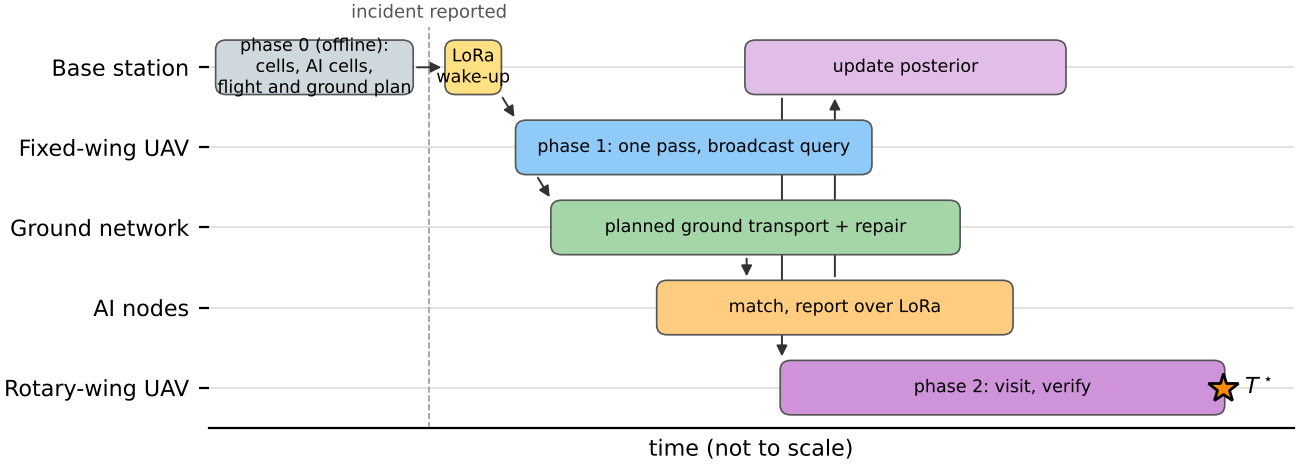
\includegraphics[width=\columnwidth]{draft2-phases-labelled.png}
\caption{Timeline of one mission. Phase~0 runs before any incident. Phase~1 overlaps the ground transport, the matching
and the LoRa reports; phase~2 can start as soon as the first report arrives. $T^\star$ is the time at which the person
is confirmed.}\label{fig:phases}
\end{figure}

\section{Related Work}\label{sec:related}
\textbf{UAV-enabled multicasting and data collection.} Trajectories are routinely optimised jointly with communication
\cite{zeng2016mag,mozaffari2019,wu2018}. Zeng \emph{et al.} \cite{zeng2018multicast} minimise the time for every ground
terminal to recover a common file directly from a rotary-wing UAV, and name a subsequent device-to-device sharing phase
as future work. Data collection from sensor networks, the reverse direction, jointly designs the wake-up schedule and
the trajectory \cite{zhan2018}, or clusters the sensors and plans multi-UAV tours under endurance constraints
\cite{nguyen2023gambac}. We consider a fixed-wing UAV that cannot dwell, receivers that are a known subset of a
multi-hop 802.15.4 mesh, and ground cooperation planned from the trajectory before take-off.

\textbf{Dissemination and routing in sensor networks.} Deluge \cite{hui2004} and Trickle \cite{levis2004} spread an
object by advertise--request epidemics; Typhoon \cite{liang2008}, Splash \cite{doddavenkatappa2013} and Pando
\cite{du2017} speed this up with channel switching, constructive interference and fountain codes. All of them start
from a sink and target every node. Minimum-latency broadcast scheduling \cite{you2013} asks for the shortest schedule
that informs all nodes under interference, with one source. Our transport differs in where the data enters (a known
segment at every cell under the track), in whom it targets (a few AI cells) and in that the plan follows from the
flight. Routing around holes with balanced load \cite{nguyen2021hole} is related to routing around cells without
devices, e.g., rivers and clearings.

\textbf{Forest networks and channels.} GreenOrbs \cite{liu2013greenorbs} measured a large 802.15.4 network in a
forest; networked camera traps \cite{kissling2024} and wildfire meshes \cite{dryad} are the deployments closest to ours.
Foliage loss at microwave frequencies is modelled empirically \cite{weissberger1982,itu833}; field tests of 2.4\,GHz
802.15.4 links from UAVs report ranges well below nominal and an altitude optimum near 45\,m \cite{nekrasov2019}.

\textbf{Curvature-constrained routing.} The Dubins TSP is NP-hard \cite{leny2012}; with neighbourhoods it is solved in
practice by sampling entry configurations and transforming the generalised TSP into an asymmetric TSP
\cite{isaacs2011,noon1993,obermeyer2009}. Our tours use these building blocks, but the objective is the readiness time
of the ground transport rather than tour length.

\textbf{Search theory and lost-person behaviour.} The optimal searcher path problem is NP-hard
\cite{trummel1986}; the minimum latency problem, its deterministic counterpart, is NP-hard even on weighted trees
\cite{sitters2002}; expanding search, where the searched region grows from a root, admits exact and approximation
algorithms \cite{hermans2019}. Lost-person statistics give the distance from the last-seen point by subject category
\cite{koester2008,koester1998}. We use these results to model the prior of phase~2 and to place (P2).
